\begin{figure*}[t]
    \centering
    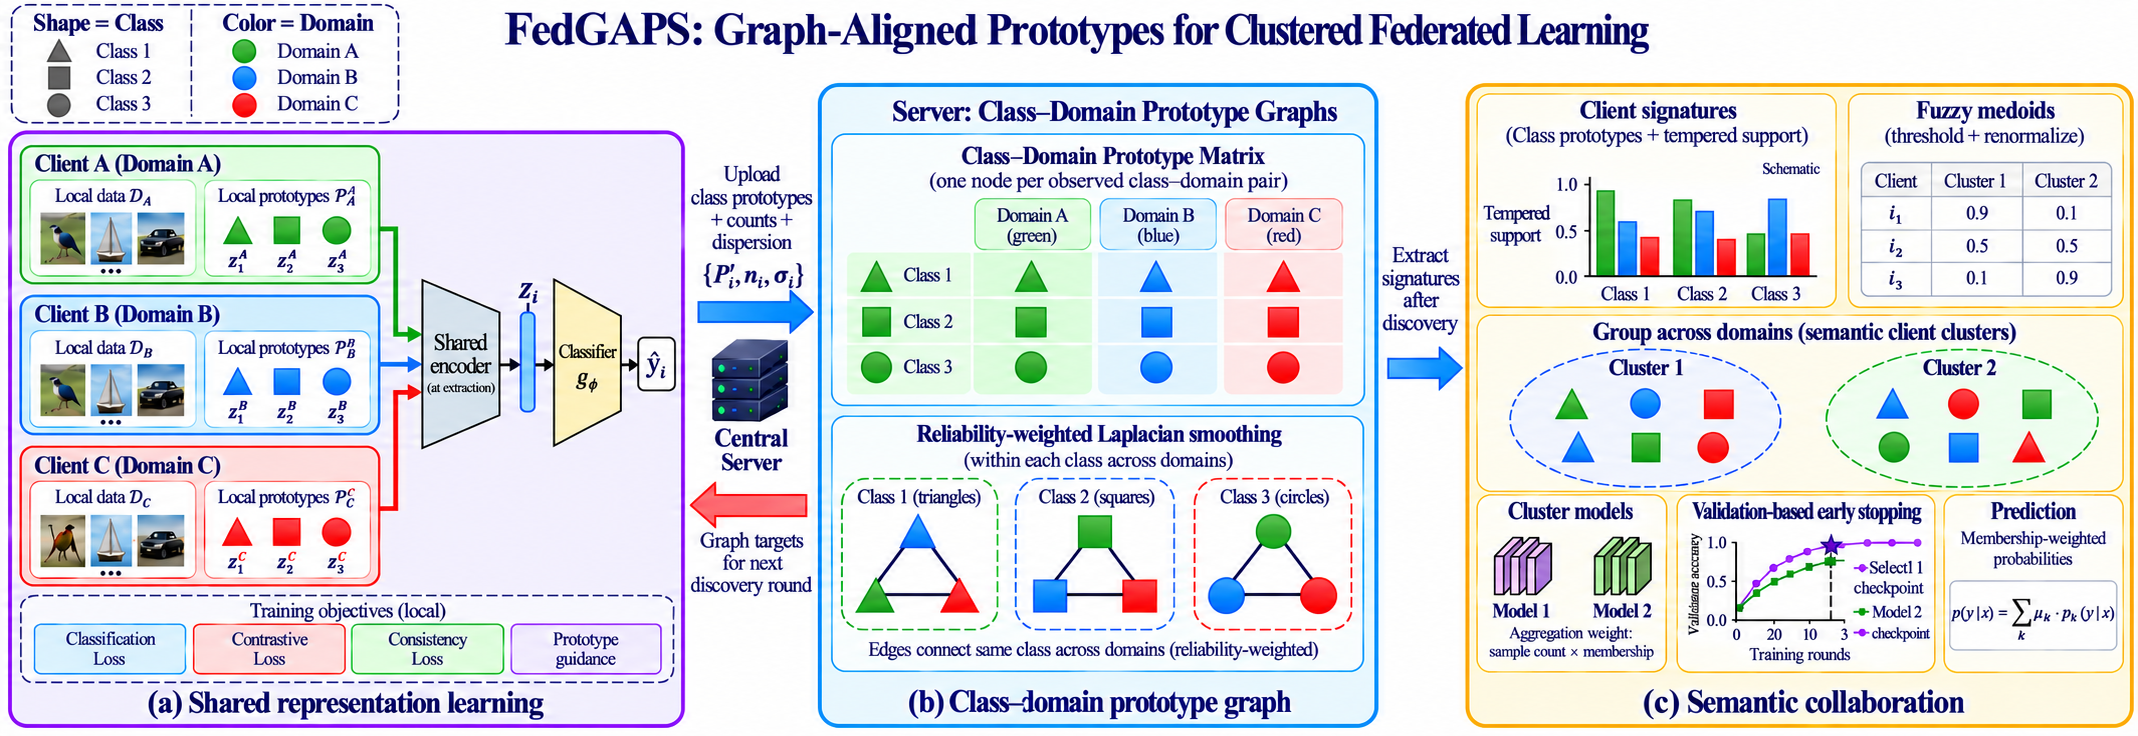
\includegraphics[width=\textwidth]{docs/assets/overview.png}
    \caption{\textbf{Overview of FedGAPS.}
    Shapes denote classes and colors denote acquisition domains.
    \textbf{(a)} Clients learn a shared discovery representation and compute
    class prototypes with support and dispersion statistics.
    \textbf{(b)} The server aggregates prototypes within class--domain pairs
    and constructs same-class cross-domain graphs. Reliability-weighted graph
    smoothing produces prototype targets that guide subsequent local
    representation learning.
    \textbf{(c)} Clients extract signatures from the learned shared encoder.
    Reliability-tempered signature comparisons yield fuzzy memberships,
    which guide cluster-specific training and prediction. Validation-based
    early stopping selects a checkpoint separately for each cluster.
    The illustrated memberships and learning curves are schematic.}
    \label{fig:overview}
\end{figure*}
